\documentclass[a4paper,12pt]{article}
\usepackage{CJKutf8}
\usepackage{amsthm}
\usepackage{amsmath}
\usepackage{amssymb}
\usepackage{geometry}
\usepackage{tikz}

% 边距
\geometry{left=2.0cm,right=2.0cm,top=2.0cm,bottom=3.0cm}

% 大题
\newenvironment{firstlayer}{\begin{list}{}{\renewcommand{\makelabel}[1]{\textbf{##1}.\hfil}}}{\end{list}}

% 小题
\newenvironment{secondlayer}{\begin{list}{}{\renewcommand{\makelabel}[1]{(##1)\hfil}}}{\end{list}}

\newtheorem{theorem}{Theorem}
\newtheorem{lemma}[theorem]{Lemma}
\newtheorem{proposition}[theorem]{Proposition}
\newtheorem{corollary}[theorem]{Corollary}
\newtheorem{exercise}{Exercise}
\newtheorem*{solution}{Solution}
\newtheorem{definition}{Definition}
\theoremstyle{definition}

\makeatletter \renewenvironment{proof}[1][Proof] {\par\pushQED{\qed}\normalfont\topsep6\p@\@plus6\p@\relax\trivlist\item[\hskip\labelsep\bfseries#1\@addpunct{.}]\ignorespaces}{\popQED\endtrivlist\@endpefalse} \makeatother
\makeatletter
\renewenvironment{solution}[1][Solution] {\par\pushQED{\qed}\normalfont\topsep6\p@\@plus6\p@\relax\trivlist\item[\hskip\labelsep\bfseries#1\@addpunct{.}]\ignorespaces}{\popQED\endtrivlist\@endpefalse} \makeatother

% 大题
\newenvironment{problems}{\begin{list}{}{\renewcommand{\makelabel}[1]{\textbf{##1}\hfil}}}{\end{list}}

% 小题
\newenvironment{steps}{\begin{list}{}{\renewcommand{\makelabel}[1]{(##1)\hfil}}}{\end{list}}

% 标题
\title{Project 1}
\author{Zilong Li\\\small Student ID: 518070910095}
\date{\today}

\begin{document}
\maketitle

\noindent\textbf{Warmups}

\begin{problems}
    \item[1] All horses are the same color; we can prove this by induction on the number of horses in a given set. Here's how: If there's just one horse then it's the same color as itself, so the basis is trivial. 
    For the induction step, assume that there are $n$ horses numbered 1 to $n$. By the induction hypothesis, horses 1 through $n - 1$ are the same color, and similarly horses 2 through $n$ are the same color. 
    But the middle horses, 2 through $n - 1$, can't change color when they're in different groups; these are horses, not chameleons. 
    So horses 1 and $n$ must be the same color as well, by transitivity. Thus all $n$ horses are the same color; QED." What, if anything, is wrong with this reasoning?
    \begin{solution}
        \textbf{It is wrong.} In fact, the definition of \emph{same} is not exact for $n=1$ senario. The \emph{same} should describe the relationship between two \emph{different} objects. The mathematical induction should start from $n=2$.

        For $n=2$, \emph{the middle horses} are not existed (from 2 through $n-1=1$). The basis step does not holds.
    \end{solution}

    \item[2] Find  the  shortest  sequence  of  moves  that  transfers  a  tower  of $n$ disks from the left peg $A$ to the right peg $B$, if direct moves between $A$ and $B$ are disallowed. (Each move must be to or from the middle peg. As usual, a larger disk must never appear above a smaller one.)
    
    \item[3] Show that, in the process of transferring a tower under the restrictions of the preceding exercise, we will actually encounter every properly stacked arrangement of $n$ disks on three pegs.
    
    \item[4] Are there any starting and ending congurations of $n$ disks on three pegs that are more than $2n-1$ moves apart, under Lucas's original rules?
    
    \item[5] A ``Venn diagram'' with three overlapping circles is often used to illustrate the eight possible subsets associated with three given sets:
    
    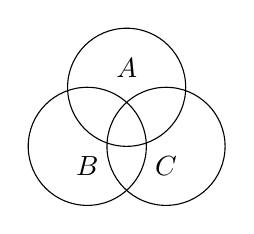
\begin{tikzpicture}[scale=0.5]
\draw  (-2,3.5) node[above] {$A$}  ellipse (1.5 and 1.5);
\draw  (-3,2) node[below] {$B$} ellipse (1.5 and 1.5);
\draw  (-1,2) node[below] {$C$} ellipse (1.5 and 1.5);
\end{tikzpicture}


    Can the sixteen possibilities that arise with four given sets be illustrated by four overlapping circles?
\end{problems}

\end{document}
